% Findings of the Fano/dispersion investigation (2026-08-04..08).
% Standalone-compilable draft section material for the next paper.
%   pdflatex fano_findings.tex   (figures in ./figs/)
\documentclass[11pt]{article}
\usepackage[margin=1in]{geometry}
\usepackage{amsmath,amssymb}
\usepackage{booktabs}
\usepackage{graphicx}
\usepackage{caption}
\usepackage[colorlinks=true,linkcolor=blue,citecolor=blue]{hyperref}

\newcommand{\ssppp}{\textsc{ss2p2}}
\newcommand{\lgm}{\textsc{lgm}}
\newcommand{\Fano}{F}

\title{Closing the Dispersion Gap in Neural Limit-Order-Book Simulators:\\
Findings from the August 2026 Fano Investigation}
\author{Honglin Fu}
\date{August 2026 (working notes)}

\begin{document}
\maketitle

\begin{abstract}
We investigate why neural marked-temporal-point-process (MTPP) simulators of
limit-order-book (LOB) order flow under-disperse --- their simulated event
counts exhibit Fano factors far below real markets --- and what repairs the
gap. Across six experimental arms on three Coinbase assets we find:
(i) the bounded-rate \ssppp{} head, as trained, is not reliably self-exciting
(measured impulse responses are sign-inconsistent and saturated);
(ii) one-step maximum likelihood systematically misallocates excitation
kernel spectra away from dispersion-relevant timescales (three independent
demonstrations); (iii) covering the measured scales with the training window
(seq $1024\!\to\!4096$) converts the Fano profile from a seed lottery into a
reproducible, near-real rise --- the largest single improvement found;
(iv) at equal training budget a dispersion/accuracy frontier exists
\emph{along the training trajectory of a single model}: dispersion peaks
early, accuracy peaks late, and no likelihood-selected checkpoint attains
both; and (v) the residual level offset is dominated by rate-ceiling
saturation ($33\%$ of events at the cap), not by amplitude learning or
closed-loop drift. We situate these results against Jain's Compound-Hawkes
programme, whose moments-based calibration targets cross-scale count
covariances by construction, and derive a certified route (linear Hawkes
ground with pinned rate and settable branching) for which dispersion is a
parameter rather than an emergent hope.
\end{abstract}

\section{Framing: two identities}
For bucketed counts $N_\Delta$ over windows of width $\Delta$, the Fano
factor is $\Fano(\Delta)=\operatorname{Var}(N_\Delta)/\mathbb{E}[N_\Delta]$.
Two identities organize the investigation.

\paragraph{Cox decomposition.} Conditioning on the intensity path, with
$\Lambda_\Delta=\int_\Delta\lambda\,dt$,
\begin{equation}
\Fano(\Delta) \;=\; 1+\frac{\operatorname{Var}(\Lambda_\Delta)}{\mathbb{E}[\Lambda_\Delta]}.
\label{eq:cox}
\end{equation}
All excess dispersion is variance of the integrated intensity. A post-hoc
rescaling $\lambda\!\to\!\kappa\lambda$ moves $\Fano-1$ only linearly with the
rate: once the mean is calibrated, dispersion is fully determined by the
model's relative intensity-fluctuation structure.

\paragraph{Branching form.} For a subcritical linear Hawkes process with
branching ratio $n$, cluster sizes $S$ satisfy $\mathbb{E}[S]=(1-n)^{-1}$ and
$\mathbb{E}[S^2]=(1-n)^{-3}$, whence
\begin{equation}
\Fano(\infty)\;=\;\frac{\mathbb{E}[S^2]}{\mathbb{E}[S]}\;=\;\frac{1}{(1-n)^2}.
\label{eq:branching}
\end{equation}
The \emph{rising} profile $\Fano(\Delta)$ across $\Delta$ is the fingerprint of
long-memory (power-law-like) intensity autocovariance; single-exponential
kernels plateau.

\paragraph{Empirical targets.} Real Coinbase order flow (7 days, Jan 2026):
$\Fano(1\mathrm{s})\!\approx\!40$--$70$ rising to $\Fano(50\mathrm{s})\approx
394$ (SOL), $1247$ (ETH), $1463$ (BTC), still rising at the window edge.
Implied branching (lower bounds): $n\approx0.948$ (SOL), $0.971$ (ETH),
$0.973$ (BTC). By Eq.~\eqref{eq:branching} the seemingly small difference
$0.948\!\to\!0.973$ quadruples asymptotic dispersion.

\section{Asset heterogeneity: a tick-regime contrast}
\label{sec:assets}
\begin{table}[h]\centering\small
\begin{tabular}{lrrrrr}
\toprule
 & trades (7d) & book rows & rows/trade & rate (ev/s) & 1024-ev window \\
\midrule
BTC & 41{,}675 & 52.9M & 1268 & 40.6 & $\sim$25\,s \\
ETH & 94{,}048 & 55.5M & 590 & 42.8 & $\sim$24\,s \\
SOL & 40{,}048 & 20.1M & 501 & 22.3 & $\sim$46\,s \\
\bottomrule
\end{tabular}
\caption{Raw data volumes and stream speeds (Coinbase spot, 2026-01-01..07).}
\end{table}

Event-type composition differs qualitatively: inside-spread (IS) limit orders
are $52\%$ of BTC events, $34\%$ of ETH, but only $7\%$ of SOL, whose flow is
instead cancel-dominated ($43\%$ CO). BTC/ETH are \emph{small-tick} assets in
Bouchaud's sense (price-priority undercutting wars inside a multi-tick
spread---the most self-exciting flow); SOL is effectively \emph{large-tick}
(1-tick spread, queue-priority churn). This microstructural contrast, not
only the rate difference, explains the criticality ordering and why every
simulator finds SOL easiest; it matches Jain's thesis (Ch.~3) where stylized
facts scale systematically with relative tick size.

\section{Mechanism: the bounded head is not reliably self-exciting}
\label{sec:mechanism}
\ssppp{} factorizes intensity into a softmin-bounded scalar rate
$\lambda(t)=s\,\mathrm{softplus}\!\big(c-\mathrm{softplus}(c-w^{\top}h(u))\big)
\le s\,\mathrm{softplus}(c)$ and rate-neutral softmax marks. Stability is a
bound on the rate \emph{level}; nothing constrains the sign or magnitude of
the event$\to$intensity feedback.

Measuring the literal expected-offspring count (inject one extra event into a
real history; integrate the additional intensity mass over 20\,s) across six
trained checkpoints: the median response is $\approx 0$ \emph{to negative}
($-8.7$ to $+0.2$ across seeds), positive in only 27--56\% of states, with
sign flips across seeds. Post-event intensity is pinned at the ceiling in
every window. The model's residual dispersion arises from a stereotyped
impulse--decay envelope, not compounding cascades; cascades cannot compound
because the second event in a burst adds nothing the first did not.

\section{Experimental arms}
All arms use the \texttt{ma\_cbse} protocol: 62-channel event streams, TBPTT,
categorical marks, streaming next-event evaluation on every test event,
validation-calibrated 600\,s rollouts, 3 training seeds $\times$ 3 rollout
seeds per asset.

\subsection{Negative and diagnostic arms}
\begin{itemize}
\item \textbf{Book-state conditioning} (\texttt{ss2p2-lob}; six top-10-ladder
  summary features): prediction unchanged (BTC accuracy $0.4484$ vs
  $0.4478$); closed-loop simulation \emph{worse} on volatility-structure
  facts. Conditioning on self-replayed book state becomes a smoothing
  feedback path. Consistent with the world-agent literature
  (Coletta et al.), which likewise conditions only on low-dimensional
  summaries.
\item \textbf{\lgm{}} (linear Hawkes ground $\times$ \ssppp{} marks on the
  shared backbone): $\lambda_k=(\mu_0+\sum_m a_m S^m(t))\,
  \mathrm{softmax}(z_k(u))$ with exact branching $n=\sum_m a_m/\beta_m$
  (hard-projected) and the \emph{rate pin} $\mu_0=R(1-n)$, which makes the
  free-rollout mean rate exact by construction (calibration finds
  $\kappa=1.01$, vs $\kappa\approx0.52$ for \ssppp{}). Two methodological
  findings: (a) ground accumulators must cold-start at their stationary mean
  $\mathbb{E}[S^m]=R/\beta_m$ (zero cold-starts bias windowed validation
  against slow-memory solutions; best-model selection then freezes runs at
  epoch~1 --- observed on all nine initial runs); (b) with the fix, marks
  reach near-parity ($0.186$ vs $0.192$ on SOL) while the 8-parameter clock
  costs $0.68$ nats of timing likelihood. Fano: correct rising shape,
  seed spread $\pm2$ at 50\,s (vs $\pm217$ for \ssppp{}) --- dispersion as a
  property of certified parameters --- but low level under $n=0.95$.
\item \textbf{Typed kicks, wider kernel bank} (\texttt{lgm-k}; per-channel
  kicks $w_k$, $M{=}6$ log-spaced kernels, $n=0.97$): prediction improved to
  best-in-class on SOL ($0.1967$), but MLE moved kernel mass to
  $\beta\approx0.008$ ($\sim$2-minute memory), pushing variance beyond the
  observation window; $\Fano$ \emph{regressed}. Third independent
  demonstration that one-step likelihood misallocates the spectrum.
\item \textbf{Dispersion-matching loss} (\texttt{ss2p2-disp}; match
  $1+\operatorname{Var}(\Lambda_\Delta)/\mathbb{E}[\Lambda_\Delta]$ to the
  batch-empirical Fano at $\{0.5,2,8\}$\,s): pins the level at trained scales
  reproducibly, \emph{flat beyond the grid}; teacher-forced variance matching
  is not closed-loop compounding. A raised cap ($c{=}12$) produced the
  documented near-critical calibration fragility on one seed.
\end{itemize}

\subsection{The window-coverage result (headline)}
\label{sec:w4k}
At seq~1024, TBPTT gradients truncate at $\sim$24--25\,s on BTC/ETH ---
before the 20--50\,s scales where their simulated profiles flatten; SOL's
$\sim$46\,s windows cover the range, and SOL was the only asset where
real-like rises appeared reliably. Setting seq/stride $=4096$
($\sim$100\,s windows) with an otherwise identical recipe:

\begin{table}[h]\centering\small
\begin{tabular}{lccc}
\toprule
BTC, per seed & seq 1024 (12 ep) & seq 4096 (12 ep) & real \\
\midrule
$\Fano(50\mathrm{s})$, s1/s2/s3 & 29 / 50 / 361 & \textbf{901 / 270 / 744} & 1463 \\
rise $\Fano(50)/\Fano(1)$ & $\times$2.5--13.9 & $\times$15--32 & $\times$20.9 \\
\bottomrule
\end{tabular}
\caption{Window coverage transforms the BTC Fano profile: all three seeds
rise steeply (best seed within $1.6\times$ of real at 50\,s). ETH: 2/3 seeds
transformed. SOL: unchanged (negative control --- its windows already covered
the measured scales).}
\label{tab:w4k}
\end{table}

\begin{figure}[h]\centering
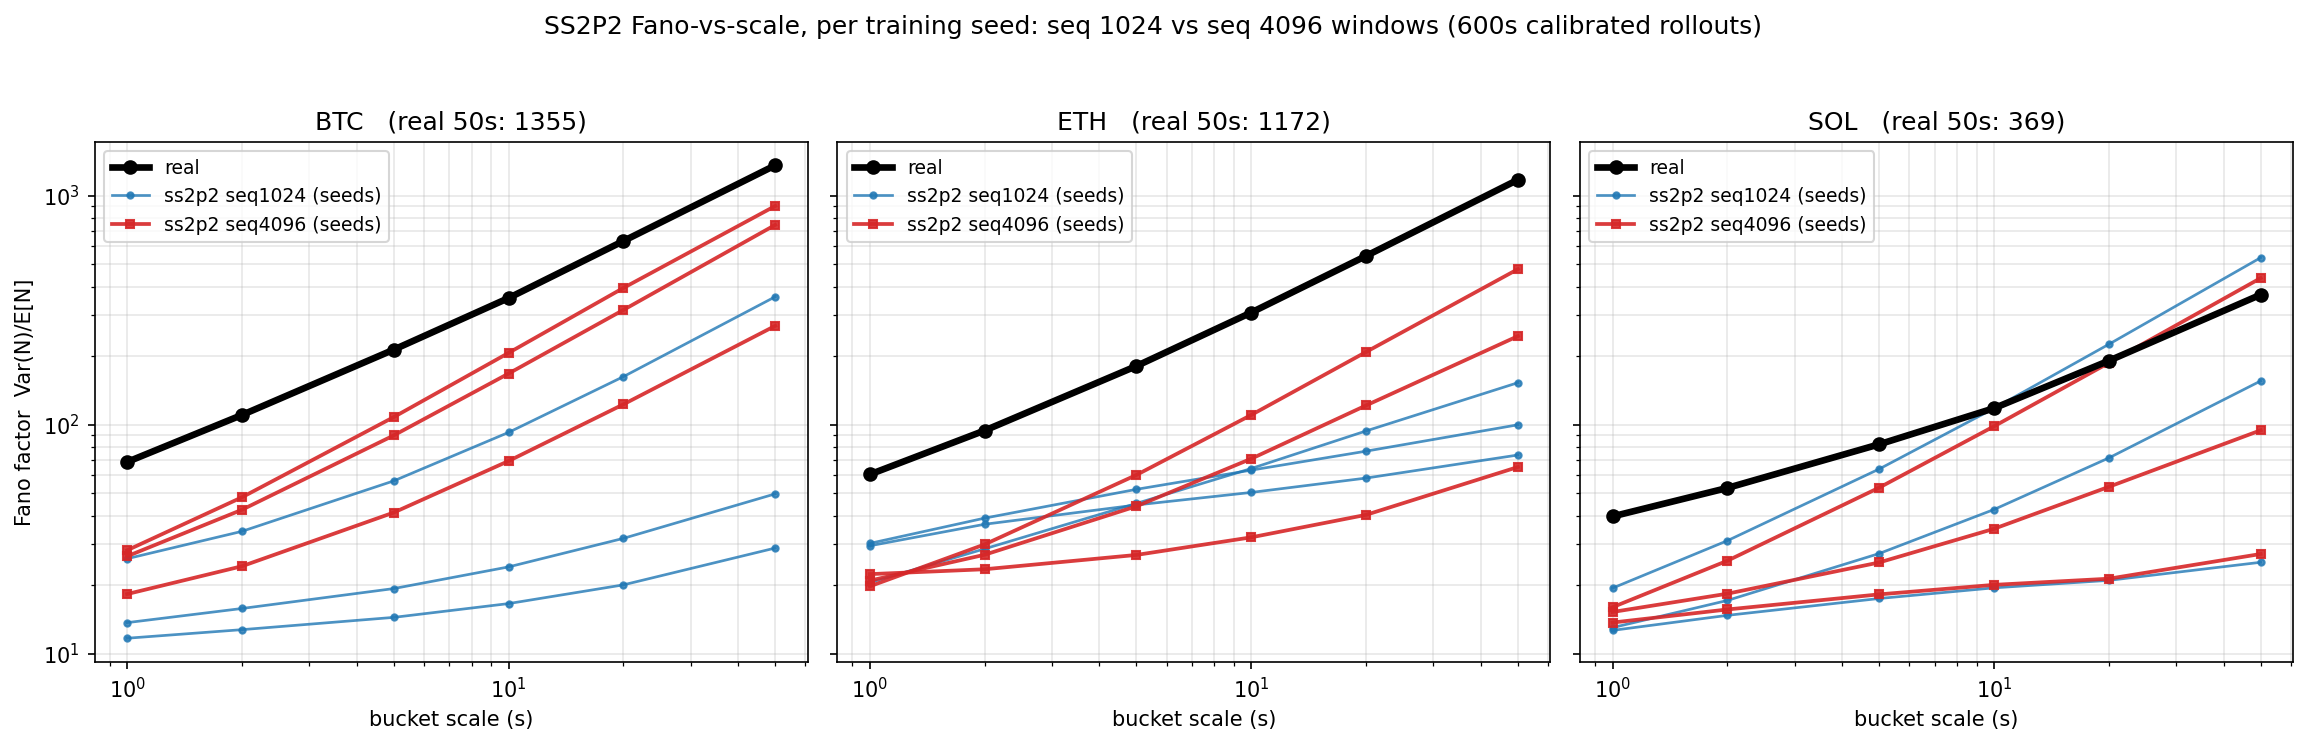
\includegraphics[width=\textwidth]{figs/fano_w4k.png}
\caption{Per-seed Fano-vs-scale (log--log): real (black), seq-1024 seeds
(blue), seq-4096 seeds (red).}
\end{figure}

\subsection{Equal-budget controls: a dispersion/accuracy frontier along the
training path}
\label{sec:frontier}
seq~4096 with matched stride quarters the updates per epoch; 48 epochs
restores the baseline's total update count exactly.

\begin{table}[h]\centering\small
\begin{tabular}{lccc}
\toprule
BTC & accuracy & $\Fano(1\mathrm{s})$ & $\Fano(50\mathrm{s})$ per seed \\
\midrule
base (1024, 12 ep) & 0.4478 & 17.1 & 29, 50, 361 \\
w4k (4096, 12 ep) & 0.4183 & 24.3 & \textbf{901, 270, 744} \\
w4k48 (4096, 48 ep) & \textbf{0.4514} & 16.6 & 232, 87, 230 \\
w4kd ($+$disp.\ loss, 48 ep) & \textbf{0.4519} & 11.1 & 52, 43, 43 \\
\midrule
real & --- & 70.0 & 1463 \\
\bottomrule
\end{tabular}
\caption{Equal-updates controls on BTC (ETH/SOL analogous). Accuracy fully
recovers --- long windows are strictly better predictors at matched budget ---
but continued likelihood training walks the model away from the
burst-faithful solution it passed through at 12 epochs.}
\label{tab:frontier}
\end{table}

\noindent\textbf{Finding.} Along the MLE trajectory of a single model,
dispersion peaks early and accuracy peaks late; no likelihood-selected
checkpoint attains both. The prediction/simulation tension long observed
\emph{across} architectures exists \emph{within one training run}. The
dispersion loss under a tight cap converges all seeds to the smooth solution
(best accuracy, worst dispersion), as predicted by the saturation diagnostic
below.

\subsection{Locating the residual offset}
On the best w4k checkpoint (BTC): the dominating rate is $359$\,ev/s and the
event-time intensity distribution has $p_{50}=224$, $p_{90}=357$,
$p_{99}=358$ --- $32.8\%$ of events occur above $0.9\times$ the ceiling.
Teacher-forced on real histories, the model-implied $\Fano$ is only
$1.2$--$1.4\times$ below real at every scale (e.g.\ $240$ vs $290$ at
50\,s). The remaining level gap is therefore primarily \emph{ceiling
saturation} (which also kills the gradients of any dispersion objective),
secondarily closed-loop drift; it is not an amplitude-learning failure. A
moderate cap raise ($c{=}9$) on the equal-budget recipe is the decisive
pending control.

\section{The Jain reference point}
Jain's Compound-Hawkes programme (FRL 2024; thesis Ch.~4) never optimizes or
reports the Fano factor; dispersion realism is scored by volatility signature
plots and $|r|$-autocorrelation, and his own signature plots undershoot the
empirical level by $2$--$3\times$ --- shape, not level, is the published
state of the art. His dispersion derives from the estimator, not from
likelihood: (i) kernels are fit by Kirchner-style binned-count least squares
on a linear-log lag grid --- an autoregression of current bin counts on
lagged counts of every type, i.e.\ a moments fit whose target \emph{is} the
cross-scale count covariance; (ii) power-law kernels win AIC selection 100\%
of the time (straight lines over six decades of lag); (iii) the kernel-norm
matrix eigenvalue is capped at 1 by rescaling (a matrix
\texttt{project\_subcritical}); (iv) baselines are derived, not fitted:
$\boldsymbol{\mu}=(\mathbb{I}-\boldsymbol{M})\boldsymbol{\Lambda}$ --- the
matrix form of the \lgm{} rate pin; (v) compound order sizes (Dirac spikes at
round numbers $+$ geometric) matter enormously for price-domain dispersion
(constant-size ablation wrong by $\sim$$100\times$); (vi) a U-shaped
time-of-day multiplier.

His RL chapter converts stylized facts into functional requirements for a
market-making simulator, ranked by ablation evidence: intensity features
(the clustering state) are the agent's most valuable observable (removing
them: Sharpe $+31.5\to-20/-51$); relative queue position is next (removal
yields manipulative or unprofitable policies); and impact-memory
mis-specification \emph{manufactures} strategies --- exponential kernels
admit dynamic arbitrage that the optimizer finds (``pump and dump''),
rarely so under power-law kernels. Absence of dynamic arbitrage is
effectively a required stylized fact for RL environments.

\section{Conclusions}
\begin{enumerate}
\item Prediction and simulation are different objectives; one-step MLE is
  blind to, and repeatedly misallocates, the kernel spectrum controlling
  $\Fano(\Delta)$ --- and (\S\ref{sec:frontier}) trades dispersion away
  \emph{within} a single training run.
\item The training window must cover the measured scales
  (\S\ref{sec:w4k}): the cheapest large improvement found, converting the
  BTC profile from seed lottery to reproducible near-real rise.
\item The rate ceiling is the binding level constraint on the best current
  models ($33\%$ saturation); dispersion objectives are inert without
  headroom.
\item Certified dispersion requires linear-in-history structure: only the
  \lgm{} ground offers a settable $n$, a pinned mean rate, and closed-form
  $\Fano(\Delta)$ at any horizon. The Kirchner binned regression is the
  proven recipe for fitting it (typed, per asset) to cross-scale count
  covariances, post hoc, with the trained mark head untouched.
\item Targets must be per-asset: tick regime (IS share) drives criticality;
  $n$ differences of $0.025$ are $4\times$ Fano differences.
\item For the eventual market-making agent, the simulator acceptance
  checklist (after Jain Ch.~6) is: genuine clustering exposed as intensity
  state; honest queue mechanics; arbitrage-consistent impact with power-law
  memory; reactive spread/liquidity dynamics; realistic frictions.
\end{enumerate}

\paragraph{Provenance.} Experiments:
\texttt{ma\_cbse/\{btc,eth,sol\}/} tags \texttt{ss2p2-full},
\texttt{ss2p2-lob}, \texttt{lgm}, \texttt{lgm-k}, \texttt{ss2p2-disp},
\texttt{ss2p2-w4k}, \texttt{ss2p2-w4k48}, \texttt{ss2p2-w4kd},
\texttt{ss2p2-w4kc9} (pending). Code: \texttt{honglinfu98/simulation}
commits \texttt{7b97b21..88d22cc}; mirrors in \texttt{dmm\_sim/}. Full lab
log: \texttt{docs/fano\_investigation\_2026-08.md}.

\end{document}
